\section{Concurrency \buch{p.1}}
\subsection{Motivation}
\begin{itemize}
  \item Praktische Programme führen meist mehrere Arbeiten "`gleichzeitig"' aus. 
  \item Diese Nebenläufigkeit kann implementiert werden durch\ldots
  \begin{itemize}
    \item Quasi-Parallelität durch Betriebssystem $\rightarrow$ Synchronisation
    nötig, da auf gemeinsame Ressourcen zugegriffen wird
    \item Echte Parallelität durch Mehrprozessorsystem
  \end{itemize}
\end{itemize}

\subsection{Threads in CSharp \buch{p.7}}
Prozesse und Threads aus OS-Sicht:\\
\begin{center}
{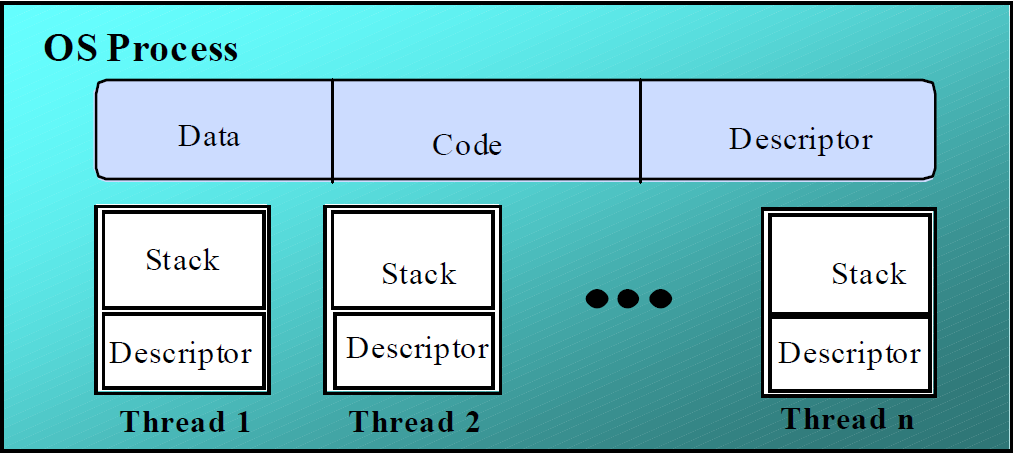
\includegraphics[width=0.5\textwidth]{images/Concurrency/ProzesseUndThreads.png}}
%\label{Fig: Schlechtes Beispiel für Modularisierung}
\end{center}
\begin{itemize}
  \item Prozess (heavyweight process):
  \begin{itemize}
    \item Code
    \item Daten
    \item Deskriptor zur Verwaltung des Prozesses durch OS (PCB, Process
    Control Block)
  \end{itemize}
  \item Thread (lightweight process):
  \begin{itemize}
    \item Teil eines Prozesses
    \item Gemeinsamer Adressraum
    \item Gemeinsame Nutzung anderer System-Ressourcen
    \item Pro Thread: Code, Stack, Deskriptor
  \end{itemize}
\end{itemize}
Ein Thread unterscheidet sich zu einem Prozess folgendermassen:\\
Man beachte: Ein Thread ist Teil eines Prozesses, das bedeutet, alles was ein
Thread inne hat, hat ein Prozess auch inne (aber NICHT umgekehrt)!\\
\begin{centering}
  \begin{tabular}{l | l}
    \hline
    \hline
    Pro Prozess vorhanden & Pro Thread vorhanden\\
    \hline
    \hline
    Adressraum & Programmzähler\\
    \hline
    Globale Variabeln & Register\\
    \hline
    Geöffnete Dateien & Stapel(Stack)\\ 
    \hline
    Kindprozesse & Zustand\\
    \hline 
    Pendente Alarme & \\
    \hline 
    Signale und Signalbehandlungsroutinen &\\
    \hline
    Buchhaltungsinformationen
  \end{tabular}
\end{centering}
Quasiparallelität:\\
Prozesse/Threads können folgende Zustände und Übergänge erfahren: 
\begin{center}
{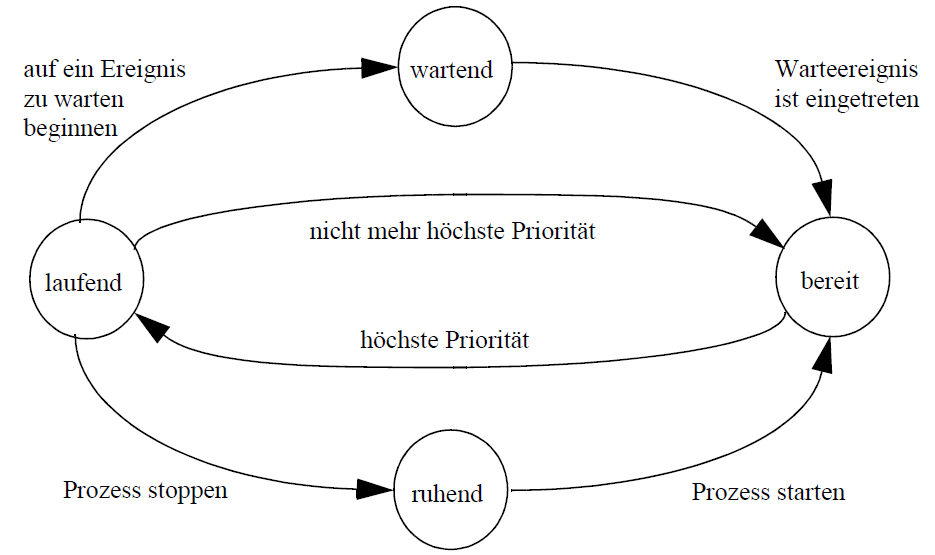
\includegraphics[width=0.5\textwidth]{images/Concurrency/Prozesszustaende.png}}
%\label{Fig: Schlechtes Beispiel für Modularisierung}
\end{center}

\begin{itemize}
  \item Threads aus Standardklasse System.Threading
  \item Jede \textbf{parameterlose void-Methode M} kann zu einem Thread gemacht
  werden 
\end{itemize}
\begin{centering}
  \begin{lstlisting}[style=C]
  Thread t = new Thread(new Threadstart(M));
  \end{lstlisting}
\end{centering}
\begin{itemize}
  \item Dem Thread-Ctor muss das Delegate \textbf{ThreadStart} übergeben werden
  \item Der Thread wird gestartet mit:  
\end{itemize}
\begin{centering}
  \begin{lstlisting}[style=C]
  t.Start();
  \end{lstlisting}
\end{centering}
\begin{itemize}
  \item Beenden des Threads: 
  \begin{itemize}
    \item Ende seiner Methode
    \item Explizierter Abrruch mitttels Abort()  
  \end{itemize} 
\end{itemize}
\begin{center}
{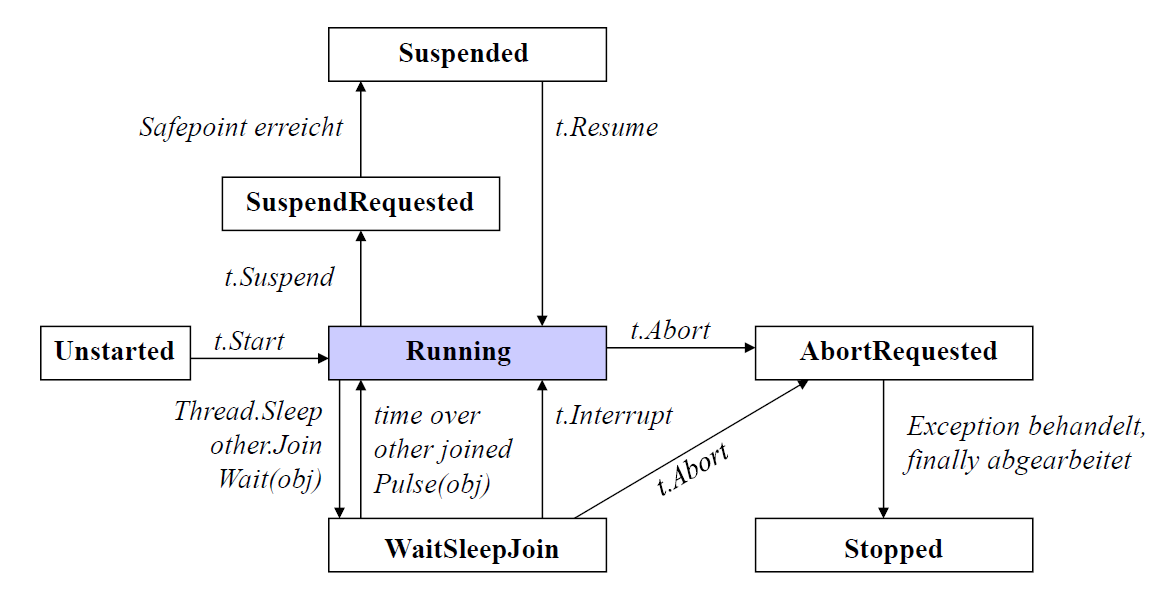
\includegraphics[width=0.5\textwidth]{images/Concurrency/Zustandsuebergaenge.png}}
%\label{Fig: Zustandübergänge}
\end{center}



\subsection{Beispiele}
Allgemeines Beispiel:
\begin{lstlisting}[style=C]
  //Zwei Programme, die staendig Zeichen auf dem Bildschirm ausgeben
  using System; 
  usign System.Threading; 
  class Printer
  {
    char ch; 
    int sleepTime; 
    public Printer(char c, int t)
    {
      ch = c;
      sleepTime = t; 
    }
    public void Print()
    {
      for(int i=0; i<100; i++)
      {
        Console.Write(ch); 
        Thread.Sleep(sleepTime); 
      }
    }
  }
  class Test
  {
    static void Main()
    {
      Printer a = new Printer('.',10);
      Printer b = new Printer('*',100);
      new Thread(a.Print).Start(); 
      new Thread(b.Print).Start();   
    }
  }
  //Das Programm laeuft so lange, bis der letzte Foreground-Thread beendet ist.
\end{lstlisting}

Beispiel für Join:
\begin{lstlisting}[style=C]
  using System; 
  usign System.Threading; 
  class Test
  {
    static void P()
    {
      for(int i=0; i<20; i++)
      {
        console.Wirte('-');
        Thread.Sleep(100);  
      }
    }
  }

  static void Main()
  {
    Thread t = new Thread(P); 
    Console.Write("start"); 
    t.Start(); 
    t.Join(); //Wartet auf t
    Console.WriteLine("end");   
  }
  //Ausgabe: start--------------------end
\end{lstlisting}
  
Threads abbrechen:
\begin{itemize}
  \item Automatisches abbrechen, sobald der Thread das Ende seiner Methode
  erreicht hat. 
  \item Ein Thread kann explizit mit Abort() abgebrochen werden
  $\rightarrow$ Dabei wird eine ThreadAbortException ausgelöst, die in der
  Thread-Methode abgefangen und behandelt werden muss. 
\end{itemize}
\begin{lstlisting}[style=C]
    using System;
    using System.Threading; 
    class Test
    {
      static void P()
      {
        try
        {
          try
          {
            try
            {
              wile(true); 
            }
            catch(ThreadAbortException)
            {
              Console.WriteLine("-- inner aborted"); 
            }
          }
          catch(ThreadAbortException)
          {
            Console.WriteLine("-- outer aborted"); 
          }
        }
        finally
        {
          Console.WriteLine("-- finally"); 
        }
      }
      
      static void Main(string[] arg)
      {
        Thread t = new Thread(P); 
        t.Start(); 
        Thread.Sleep(1); 
        t.Abort(); 
        t.Join(); 
        Console.WriteLine("done"); 
      }
    }
    //Ausgabe: 
    //-- inner aborted
    //-- outer aborted
    //-- finally
    //done
\end{lstlisting}

\subsection{Synchonisation: Zugriff auf gemeinsame Ressourcen \buch{p.20}}
Definition kritischer Bereich: 
\begin{itemize}
  \item Codebereich, in dem nebenläufige Prozesse auf gemeinsame Ressource
  zugreifen. 
  \item Zu jeder Zeit darf sich höchstens ein Prozess im kritischen Bereich
  aufhalten. 
  \item Dies wird mittels gegenseitigem Ausschluss (Mutual Exclusion, Mutex)
  sicher gestellt. 
\end{itemize}
Forderungen an die Synchronisation (Dijkstra, 1965)
\begin{itemize}
  \item Zwei Prozesse dürfen sich nicht gleichzeitig in einem kritischen Bereich
  befinden (Mutex).
  \item Über Abarbeitungsgeschwindigkeit und Anzahl Prozesse dürfen keine
  Annahmen getroffen werden. 
  \item Kein Prozess darf ausserhalb des kritischen Bereichs einen anderen
  Prozess blockieren. 
  \item Jeder Prozess, der auf den kritischen Bereich wartet, muss irgendwann
  den Abschnitt betreten dürfen (fairness condition). 
\end{itemize}


\begin{tabbing}
  \hspace*{1cm}\=\hspace*{4.2cm}\=\hspace*{3cm}\=\hspace*{2.7cm}\= \kill
  Synchro-Versuch 1\\
  \>{\bf Prozess 1} \> \> \>{\bf Prozess 2}\\
  \>\begin{lstlisting}[style=C]
      while(grant != 1)
        wait(); 
      CS; //Eintritt in Critical Section 
      grant = 2; 
    \end{lstlisting} \> \> \>
    \begin{lstlisting}[style=C]
      while(grant != 2)
        wait(); 
      CS; //Eintritt in Critical Section  
      grant = 1; 
    \end{lstlisting} \\\\
    
  Synchro-Versuch 2\\
   \>{\bf Prozess 1} \> \> \>{\bf Prozess 2}\\
   \>\begin{lstlisting}[style=C]
      while(in2)
        wait(); 
      in1 = true; 
      CS; //Eintritt in Critical Section 
      in1 = false; 
    \end{lstlisting} \> \> \>
    \begin{lstlisting}[style=C]
      while(in1)
        wait(); 
      in2 = true; 
      CS; //Eintritt in Critical Section 
      in2 = false; 
    \end{lstlisting} \\\\

  Synchro-Versuch 3\\
   \>{\bf Prozess 1} \> \> \>{\bf Prozess 2}\\
   \>\begin{lstlisting}[style=C]
        request1 = true; 
        grant = 1; 
        while(grant==1 && request2)
          wait(); 
        CS; //Eintritt in Critical Section  
        request1 = false; 
    \end{lstlisting} \> \> \>
    \begin{lstlisting}[style=C]
        request2 = true; 
        grant = 2; 
        while(grant==2 && request1)
          wait(); 
        CS;  //Eintritt in Critical Section 
        request2 = false;  
    \end{lstlisting} \\ 
\end{tabbing}

Signale:
\begin{itemize}
  \item Jeder Prozess wartet vor Betreten des kritischen Bereihs auf ein
  gemeinsames Signal. 
  \item Wenn Signal gesetzt $\rightarrow$ kritischer Bereich frei
  \item waitfor(signal) blockiert aufrufenden Prozess, falls signal nicht
  gesetzt
  \item Jeder Prozess, der fertig ist, setzt Signal mit send(signal)
  \item Mehrere Prozesse können gleichzeitig warten 
\end{itemize}

\begin{tabbing}
  \hspace*{1cm}\=\hspace*{4.2cm}\=\hspace*{3cm}\=\hspace*{2.7cm}\= \kill
  Synchronisation mit Signalen\\
  \>{\bf Prozess 1} \> \> \>{\bf Prozess 2}\\
  \>\begin{lstlisting}[style=C]
      waitFor(signal); 
      CS;  //Eintritt in Critical Section 
      send(signal); 
    \end{lstlisting} \> \> \>
    \begin{lstlisting}[style=C]
      waitFor(signal); 
      CS;  //Eintritt in Critical Section 
      send(signal); 
    \end{lstlisting} \\\\
 \end{tabbing}
 
 \subsection{Semaphoren \buch{p.30}}
 \begin{itemize}
   \item Das Signal für den Zutritt in den kritischen Bereich = Semaphor
   \item Ein Semaphor s hat zwei atomare (= nicht unterbrechbare)
     Operationen
   \begin{itemize}
     \item P(s) : Passieren $\rightarrow$ Beim Eintritt in CS (waitFor)
     \item V(s) : Verlassen $\rightarrow$ Beim Austritt aus CS (send)
   \end{itemize}
   \item Probleme bei Semaphoren
   \begin{itemize}
    \item Anwendung erfordert Disziplin
    \begin{itemize}
      \item Jedes P(s) braucht ein V(s)
      \item Probleme treten auf, wenn V(s) vergessen geht!
      \item Beim Auftreten einer Excewption kann das Freigeben ebenfalls
      schwierig sein. 
    \end{itemize}
   \end{itemize}
 \end{itemize}
 
 \subsection{Thread-Synchronisation in CSharp \buch{p.35}}
 Das Monitorprinzip
 \begin{itemize}
   \item Grundprinzip: Abstrakten Datenyp definieren, der genau die Funktionen
   in der Schnittstelle anbietet, die notwendig sind. 
   \item Der Aufrufer ruft diese Funktionen auf, er muss sich aber nicht um die
   Synchro kümmern. 
   \item Die Synchro (z.Bsp. mit Semaphoren) ist in der Implementation des
   Monitors lokal gelöst. 
   \item Problem wird einmal im Monitor gelöst, die Aufrufer müssen sich nicht
   mehr darum kümmern. 
 \end{itemize}
 
Beispiel Mutual Exclusion 
\begin{lstlisting}[style=C]
  //lock(Variable) Statement
  class Account
  {
    long val = 0; 
    public void Deposit(long x)
    {
      lock(this)
      {
        val += x; 
      }
    }
    public void Withdraw(long x)
    {
      lock(this)
      {
        val -= x; 
      }
    }
  }
\end{lstlisting} 
Lock lässt sich auf beliebiges anderes Objekt setzen
\begin{lstlisting}[style=C]
  object semaphore = new object(); 
  ...
  lock (semaphore){..critical section...}
\end{lstlisting} 
Klasse Monitor:\\
\begin{lstlisting}[style=C]
  lock(v) 
  ... ist Kurzform fuer ...
  try
  {
    Statement
  }
  finally
  {
    Monitor.Exit(v); 
  }
\end{lstlisting} 
Wenn Thread während der Ausführung von Statement mit Abort abgebrochen wird,
wird trotzdem finally ausgeführt und der monitor frei gegeben.\\

Wait und Pulse:
\begin{tabbing}
  \hspace*{1cm}\=\hspace*{4.2cm}\=\hspace*{3cm}\=\hspace*{2.7cm}\= \kill
  Beispiel:\\
  \>{\bf Thread A} \> \> \>{\bf Thread B}\\
  \>\begin{lstlisting}[style=C]
      lock(v) //1
      {
       ...
       Monitor.Wait(v); //2
       ...
      }
    \end{lstlisting} \> \> \>
    \begin{lstlisting}[style=C]
      lock(v) //3
      {
        ...
        Monitor.Pulse(v); //4
        ...
      }//6
    \end{lstlisting} \\\\
\end{tabbing}
\begin{enumerate}
   \item A kommt zu lock(v) und erhält Eintritt, da kein anderer Thread im
   gesperrten Bereich ist. 
   \item A kommt zu Wait, legt sich schlafen und gibt die Sperre frei. 
   \item B kommt zu lock(v) und erhält Eintritt, da die Sperre frei ist. 
   \item B komm tzu Pulse und weckt damit A. Es kann (aber muss nicht) ein
   Thread-Wechsel statt finden. 
   \item A versucht, die Sperre wieder zu erlangen, was aber nicht gelingt, da B
   sie noch hat. 
   \item B gibt am Ende des gesperrten bereichs die Sperre frei, A kann nun
   wiede reintreten und weiter laufen. 
\end{enumerate}
Beachte: 
\begin{itemize}
   \item Wait(v) und Pulse(v) dürfen nur in einer Anweisungsfolge aufgerufen
   werden, die mit lock(v) geschützt wurde.
   \item Zwischen Pulse(v) und dem dadurch geweckten Thread können andere
   Threads zur Ausfürhung gelangen, die in der Zwischenzeit versucht haben, die
   Sperre zu bekommen\\ $\rightarrow$ Die Bedingung von Pulse muss nach wait
   nicht mehr gelten!\\
   Daher sollte man die Wait-Bedingung immer in einer Schleife prüfen: 
\end{itemize}
\begin{lstlisting}[style=C]
  while(condition false)
    Monitor.Wait(v); 
  ...
  make condition true;
  Monitor.Pulse(v);       
\end{lstlisting}
\begin{itemize}
  \item PulseAll(v) weckt alle in v wartenden Threads, aber nur einer darf in
  den gesperrten Bereich. Der nächste darf erst rein, wenn der Vorgänger die
  Sperre frei gibt.
\end{itemize}
\begin{lstlisting}[style=C]
  class Buffer
  {
    const int size = 4; 
    char[] buf = new char[size];
    int head = 0; 
    int tail = 0; 
    int n = 0; 
    
    public void Put(char ch)
    {
      lock(this)
      {
        while(n==size)
          Monitor.Wait(this); 
        buf[tail] = ch; 
        tail = (tail+1)%size; 
        n++; 
        Monitor.PulseAll(this); 
      }
    }
    
    public char Get()
    {
      lock(this)
      {
        while(n==0)
          Monitor.Wait(this); 
        char ch = buf[head]; 
        head = (head+1)%size; 
        n--; 
        Monitor.PulseAll(this); 
        return ch; 
      }    
    }
  }      
\end{lstlisting}
Ablauf, wenn Producer schneller:\\
Put\\
Put\\
Put\\
Put\\
Get\\
Put\\
Get\\
\ldots

Ablauf, wenn Consumer schneller:\\
Put\\
Get\\ 
Put\\
Get\\
\ldots